\documentclass[12pt,a4paper]{report}
\usepackage[utf8]{inputenc}
\usepackage{amsmath}
\usepackage{algorithm}
\usepackage{algpseudocode}
\usepackage{amssymb}
\usepackage{graphicx}
\usepackage{geometry}
\usepackage[hidelinks]{hyperref}  % For clickable references
\usepackage[capitalise]{cleveref}  % For intelligent cross-referencing
\usepackage[english]{babel}

\usepackage{makecell}
\usepackage{caption}
\usepackage{array}
\usepackage{listings}
\usepackage{titlesec}
\usepackage{hyperref}
\hypersetup{
	colorlinks=true,
	linkcolor=black,
	filecolor=black,      
	urlcolor=cyan,
	citecolor=black
}

\graphicspath{{C:/Users/frabb/OneDrive - Cal Poly/Documents (Cloud)/0 CALPOLY/000Thesis/Chapters/Images/}}

\geometry{
	top=1in,
	bottom=1in,
	left=1.5in,
	right=1in
}

% Remove space before equations only
\makeatletter
\g@addto@macro\normalsize{%
	\setlength\abovedisplayskip{-10pt}
	\setlength\abovedisplayshortskip{-10pt}
}
\makeatother

% Updated list settings
\usepackage{enumitem}
\setlist[itemize]{nosep, leftmargin=*}
\setlist[enumerate]{nosep, leftmargin=*}

% Remove space before lists
\usepackage{etoolbox}
\BeforeBeginEnvironment{itemize}{\vspace{-\baselineskip}}
\BeforeBeginEnvironment{enumerate}{\vspace{-\baselineskip}}

\setlength{\parskip}{\baselineskip}
\titlespacing*{\section}{0pt}{0pt}{0pt}
\titlespacing*{\section}{0pt}{0pt}{-10pt}
\titlespacing*{\subsection}{0pt}{0pt}{-10pt}

\captionsetup[table]{skip=0pt}

\usepackage{xcolor}

\definecolor{codegreen}{rgb}{0,0.6,0}
\definecolor{codegray}{rgb}{0.5,0.5,0.5}
\definecolor{codepurple}{rgb}{0.58,0,0.82}
\definecolor{backcolour}{rgb}{0.95,0.95,0.92}

\lstdefinestyle{mystyle}{
	backgroundcolor=\color{backcolour},   
	commentstyle=\color{codegreen},
	keywordstyle=\color{magenta},
	numberstyle=\tiny\color{codegray},
	stringstyle=\color{codepurple},
	basicstyle=\ttfamily\footnotesize,
	breakatwhitespace=false,         
	breaklines=true,                 
	captionpos=b,                    
	keepspaces=true,                 
	numbers=left,                    
	numbersep=5pt,                  
	showspaces=false,                
	showstringspaces=false,
	showtabs=false,
	tabsize=2
}

\lstset{style=mystyle}

\title{Tutorial}
\author{Jakob Frabosilio}
\date{\today}
\begin{document}
	
\chapter{Introduction} \label{chap:1c}
This thesis presents the design, implementation, and testing of an inverted short baseline acoustic positioning system meant to be deployed on an autonomous underwater vehicle (AUV). All of the work in this thesis is done above-water: this project serves as a prototype for an underwater acoustic positioning system. The final chapters include recommendations for implementing this system in an underwater environment. All of the code written for this thesis is available on GitHub \cite{thesisgit}, and is written in C/C++ for modern microcontrollers.

The primary audience for this work is underwater robotics researchers and mechatronics engineering students. A mechatronics engineering background is not required to read this thesis: basic engineering knowledge is enough to understand the main points presented in this work. The systems and algorithms presented here (fast Fourier transform cross-correlation, Kalman filtering, Hooke-Jeeves search, and more) have many uses outside of marine robotics, and every system is presented with a detailed explanation of how it works. Additionally, the design and testing of a relatively-novel actuator design (stacked hexapod platform) is covered in this thesis.

All figure numbers, section numbers and citations in this document are hyperlinked; clicking the number will take you to its location in the document. The document was written in LaTeX and its source code can be found in the GitHub repository for this thesis.

This chapter serves as an introduction to the thesis, detailing the inspiration behind the project, giving an overview of alternative underwater positioning methods, and presenting a high-level overview of the work done for this research. 

\section{Project Inspiration} \label{sec:1s1}
The main inspiration for this project comes from a desire to build a remotely-operated underwater vehicle (ROV). Plenty of attempts at a “do-it-yourself” ROV have been made and are documented online \cite{cpsdrone}, and many commercial ROVs can be purchased online \cite{bluerov}. However, one problem kept coming up when these ROVs were considered: how do you know where they are underwater?

The Global Positioning System (GPS) is the primary way for determining an object’s location relative to the earth. It is used in planes, smartphones, and robotics, among other systems. It provides a relatively accurate way to determine the location of an object as long as there is line-of-sight to at least four GPS satellites; this means that GPS does not work well in buildings, tunnels, or underground (a problem that the reader is probably well-acquainted with). Underwater vehicles often have line-of-sight to GPS satellites, but radio waves (the communication method for GPS satellites) attenuate very quickly underwater; they cannot be used below the surface of the ocean \cite{surveyurpn}. Different methods for positioning underwater vehicles are explored in the following section.

After a review of underwater positioning system methods, an acoustic positioning system seemed to be the best low-cost method, and very few open-source projects attempt to implement one. The goal for this thesis is to design an acoustic positioning system for ROVs and AUVs that is low-cost, open-source, and well-documented. In particular, a system was desired whose position estimate does not drift over time (if the ROV/AUV needs to stay submerged for very long periods of time) and which does not require a manned boat to aid in positioning. This would allow the system to be used with ROVs and AUVs that travel far from the vessel or research station from which they are deployed. This system does require a GPS buoy or secondary (autonomous) vehicle on the surface of the water; this may be unacceptable for certain scenarios.

\section{Underwater Positioning Systems} \label{sec:1s2}
There are many types of underwater positioning methods, and each has benefits and drawbacks. Figure \ref{fig:upstable} compares and contrasts the most popular methods for positioning AUVs and ROVs.

\begin{figure}[htbp]
	\centering
	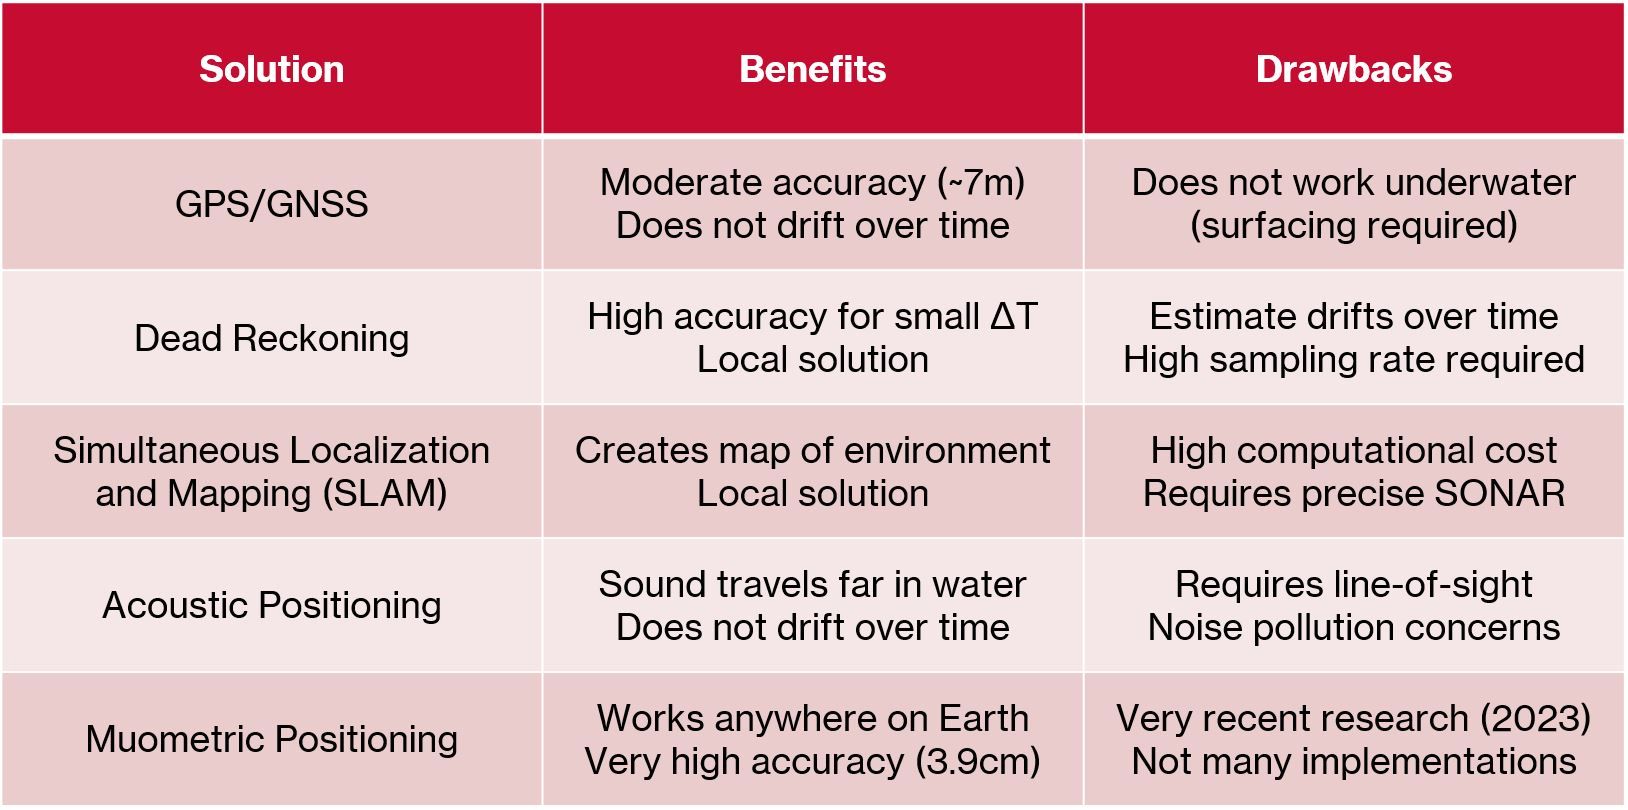
\includegraphics[width=\textwidth]{upstable}
	\caption{Common underwater positioning methods}
	\label{fig:upstable}
\end{figure}

GPS (which is a type of global navigation satellite system, or GNSS) is the most popular positioning method above-water and can be used to position AUVs when they surface. GPS uses a constellation of 31 satellites which constantly transmit their location and the time that the message was sent; from this information, a receiver can determine its position on Earth \cite{faagps}. As previously stated, GPS does not work underwater, so AUVs must come to the surface to get a new position estimate from the GPS.

Dead reckoning is a method for determining a change in position by integrating velocity and heading over time. Its history and working mechanisms are covered in detail in Section \ref{4s5}. Dead reckoning can be very accurate over small periods of time with proper equipment, but the position estimate quickly accumulates error over time. Dead reckoning is a local solution, not requiring any external satellites or vehicles, but a purely dead reckoning-based navigation system is not feasible for most scenarios. A common low-cost, low-complexity implementation is to combine GPS and dead reckoning: get a GPS position estimate at the surface, then use dead reckoning while underwater. This implementation does mean that the position estimate gets worse over time, which can be detrimental in certain scenarios.

Simultaneous localization and mapping (SLAM) is a highly-complex navigation method. It uses SONAR equipment (or cameras) to collect data about the environment, creates a map of the local environment, and then localizes itself (determines its position) within that map. For AUVs used in seafloor mapping, it is a wonderful solution since the process constructs a map of the environment. Additionally, it only uses on-board equipment and sensors - no satellites or buoys required. This means that it can only provide a position estimate within the local frame, and some other method of absolute positioning (like GPS) is required to know the position of the AUV in the global frame. This method comes with a high computational cost and requires expensive and precise equipment, but presents a unique solution to the positioning problem \cite{surveyurpn}.

Acoustic positioning is a method for determining the position of the AUV relative to a set of buoy-, seafloor-, or hull-mounted microphones. It essentially functions like an underwater GPS system, using sound waves instead of radio waves. This method does not drift over time like the previous two, but does require line-of-sight (line-of-sound?) to the underwater microphones. This method is the main focus of this thesis and is covered in depth in Chapter \ref{chap:3c}.

Finally, a brand-new underwater positioning method is muometric positioning, pioneered by Hiroyuki Tanaka. In this method, cosmic-ray muons (which bombard the Earth constantly) are detected at receiver stations, and the time-of-arrival between the receiver stations is used to determine the position of an object. Muons are capable of passing through most solid materials, meaning that the system can be used in buildings, underwater, or underground \cite{muons}. It is very new research, and is a field well-worth exploring!

\section{High-Level Overview} \label{sec:1s3}
For a single researcher, designing an acoustic positioning system and implementing it underwater is a massive task; for simplification, this system will be prototyped for above-water use. Figure \ref{fig:underwaterimp} shows how the proposed underwater system would function. A buoy with a GPS receiver is able to communicate with GPS satellites, so its position is known in the global frame. On the underside of the buoy, an acoustic transmitter sends out pulses of sound into the water beneath it. The AUV (whose position is desired) is below the buoy, within the cone of sound of the transmitter. Microphones on the body of the AUV record a pulse from the transmitter and use acoustic positioning methods to determine the location of the AUV relative to the buoy. The GPS coordinates of the buoy are encoded in the sound pulse. The AUV knows where it is relative to the buoy, and the GPS coordinates described where the buoy is relative to the global frame; this information can be combined to give the position of the AUV in the global frame. Additionally, dead reckoning is used on the AUV to supplement the acoustic position estimates. These two estimates are combined using a Kalman filter to produce the best position estimate for the AUV in the global frame.

\begin{figure}[htbp]
	\centering
	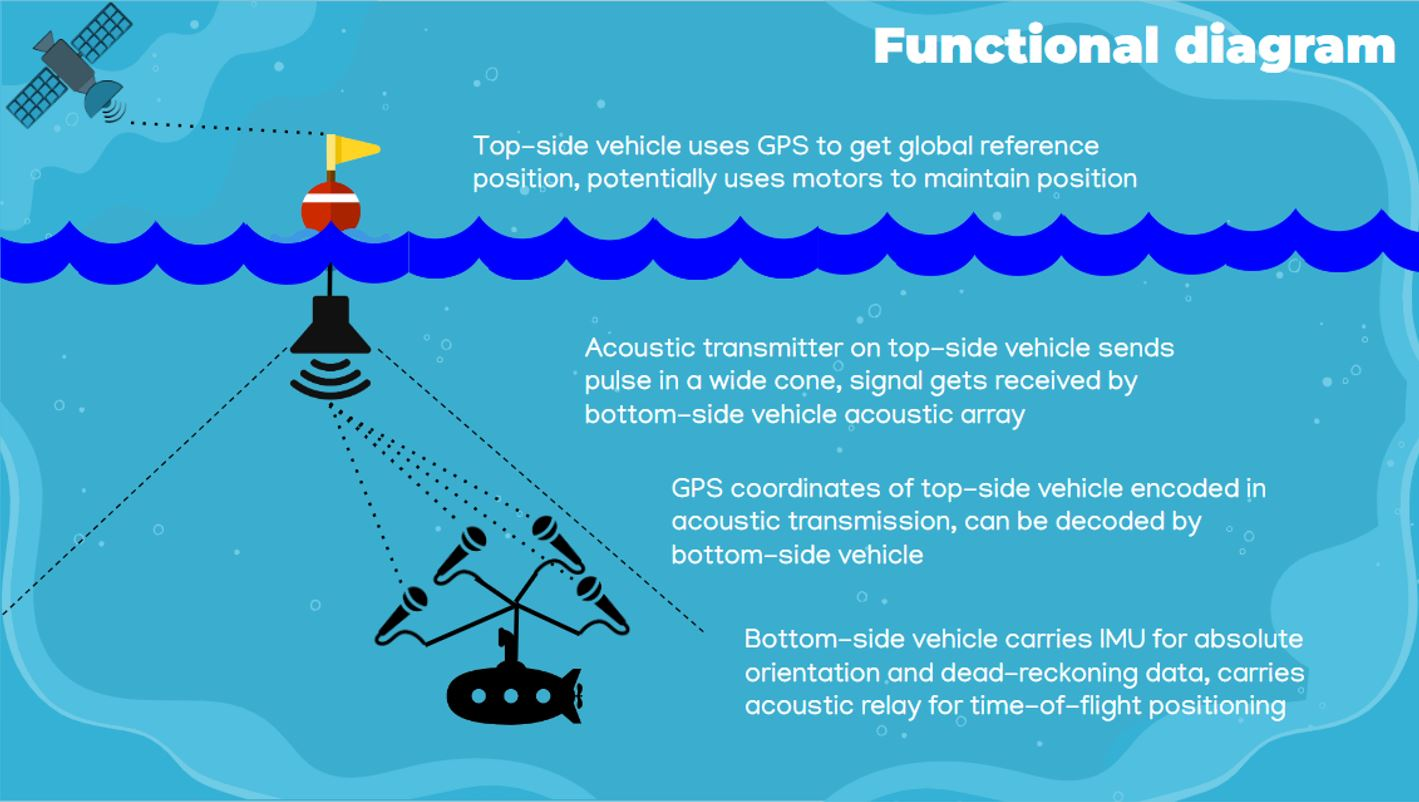
\includegraphics[width=\textwidth]{underwaterimp}
	\caption{Functional diagram for proposed underwater implementation}
	\label{fig:underwaterimp}
\end{figure}

The above-water prototype in this thesis is very similar to the proposed underwater implementation. To verify the accuracy of this system, a ground-truth positioning system is designed and fabricated; this system determines the true location of the microphone array (the above-water equivalent to the AUV). A relatively-novel actuator, a stacked hexapod platform, was used as the ground truth positioning system. The design process for the ground-truth positioning system is covered in Chapter \ref{chap:2c}.

The acoustic positioning system functions as follows: the transmitter sends out a pulse of sound, the microphones on the receiver array record the pulse, the time shift between the recordings is calculated, and the position of the transmitter relative to the receiver array is determined. This is combined with the true position of the transmitter (GPS coordinates sent over the acoustic pulse) to determine the position of the receiver array in the global frame. Chapter \ref{chap:3c} details this process.

The orientation of the receiver array / AUV must be known to transform the position estimate to the global frame. This implementation uses a Madgwick filter, a sensor fusion filter for obtaining orientation estimates using inertial measurement units (IMUs). This process, along with the implementation of a dead reckoning system, is covered in Chapter \ref{chap:4c}.

The acoustic position estimate and the dead reckoning change-in-position estimate are fused together using a Kalman filter; this process is detailed in Chapter \ref{chap:5c}, which includes an explanation of how Kalman filters work.

Finally, the system accuracy is tested and evaluated in Chapter \ref{chap:6c}, along with an extrapolation of the above-water results to the underwater regime. Chapter \ref{chap:7c} includes recommendations for improving upon the work presented in this thesis.


\bibliographystyle{IEEEtran}
\bibliography{../thesis}

\end{document}